\subsection{Overview}
\label{sect:overview}
DREAM will be used by thousands of users each day, with different needs, and located all over the Telangana region. To achieve this result and to respect all the requirements stated in the RASD, DREAM will be developed as a distributed application with clients and servers. The client will only show the graphical interface to the end-user, while the back-end will execute and support all the business logic operations. 
\begin{figure}[hbt!]
\centering
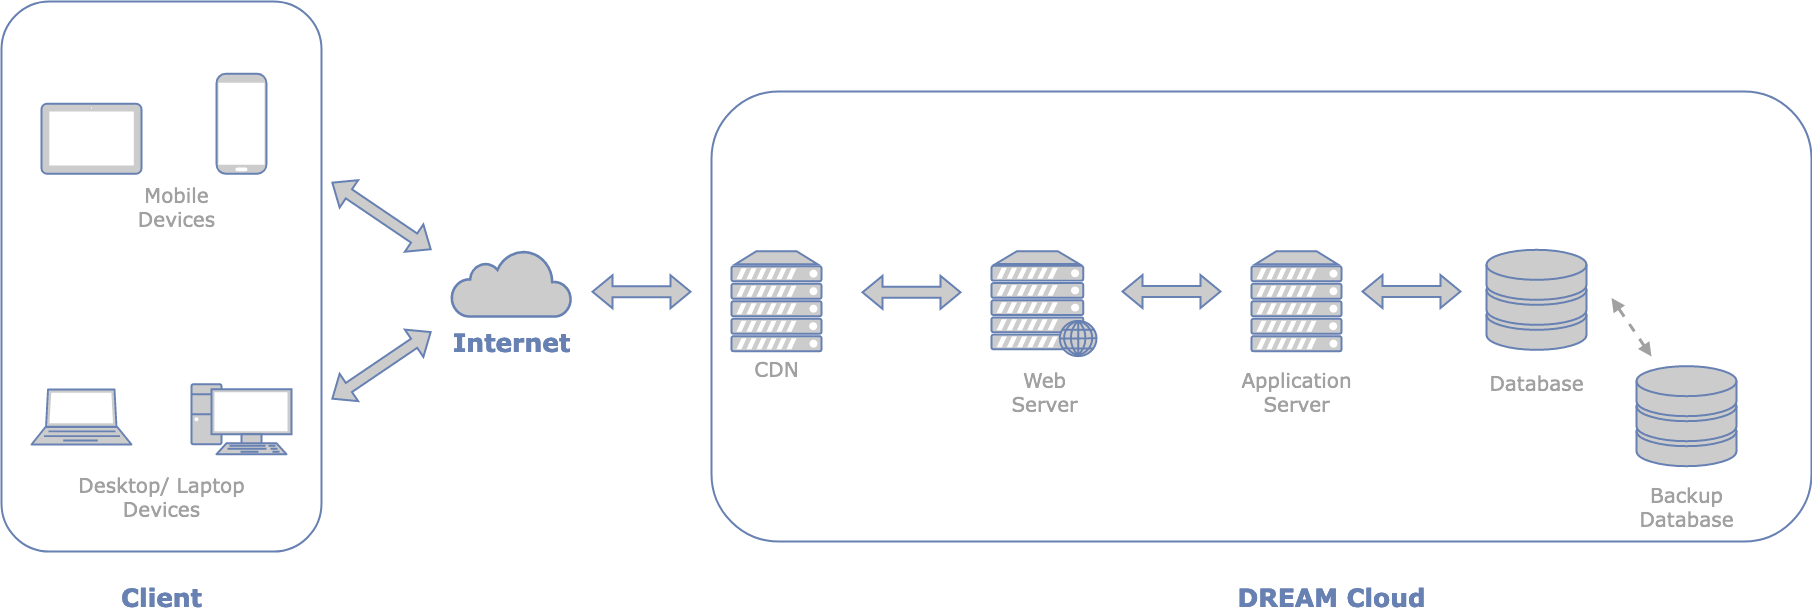
\includegraphics[width=\textwidth]{../images_diagrams/dd/highlevel_arch.png}
\caption{High-Level 5-tier Architecture.}
\label{fig:highLevelArch}
\end{figure}

\noindent
Since the application must be reliable and flexible enough in handling the growth of the user base, a cloud-based architecture is suitable for this task. In particular, DREAM Cloud is a 3-tier architecture with a web server, an application server, and a storage server (DBMS). To enable the system to always work in ideal conditions, a load balancer routes all the requests to different application servers. When the computational load exceeds the available resources, new instances of the servers are created and used to balance the extra requests. An additional tier is then placed between the user and the DREAM Cloud: a content delivery network (CDN). The CDN will relieve some load from the system and improve performances in serving static contents. Overall, the resulting application will have five tiers. Lastly, given the importance of the historical data kept inside the database, a backup system will frequently clone the data on a different server, possibly located in a different availability zone.

%\clearpage
\subsection{Component View}

The component view of the system depicts the internal structure of the DREAM system, demonstrating the components and interfaces that facilitate communication between them. The architecture consists of three different parts:
\begin{enumerate}
	\item the Agro-Farmer mobile web application which will be used by farmers and agronomists
	\item the Policy desktop web application used by policy makers
	\item the DREAM cloud that hosts the backend for all the previously introduced functionalities
\end{enumerate}
An additional element is presented for completeness: the Google Maps API is utilized by the mobile application to provide live turn-by-turn nagivation assistance. For simplicity, these three parts will be presented at different levels of abstraction, starting from the highest level, shown in Figure \ref{fig:highLevelComp}.\\

\begin{figure}[hbt!]
\centering
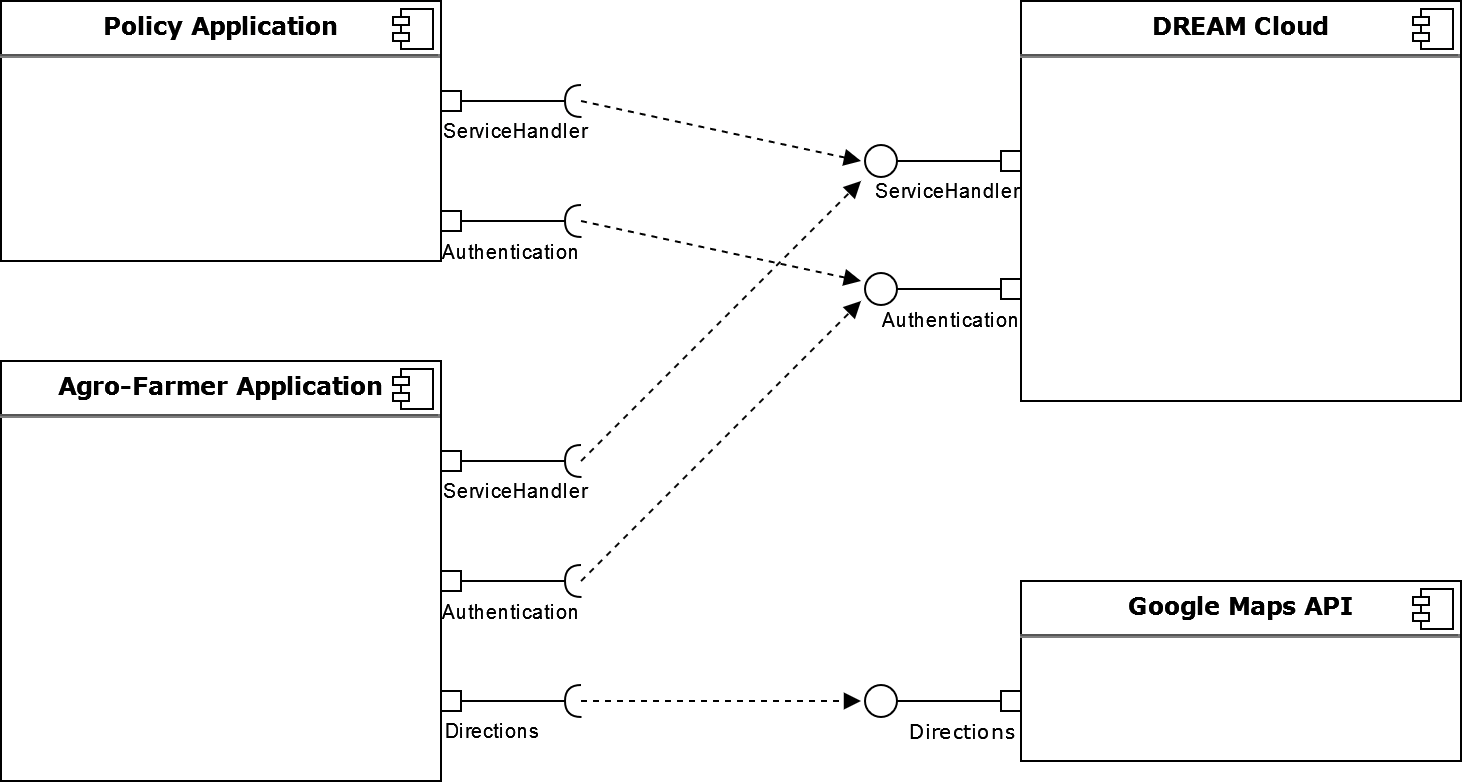
\includegraphics[width=\textwidth]{../images_diagrams/dd/high_level_cloud.png}
\caption{High-Level Component View.}
\label{fig:highLevelComp}
\end{figure}

\subsubsection{DREAM Cloud Component} \label{sect:cloudComponent}

\begin{figure}[hbt!]
\centering
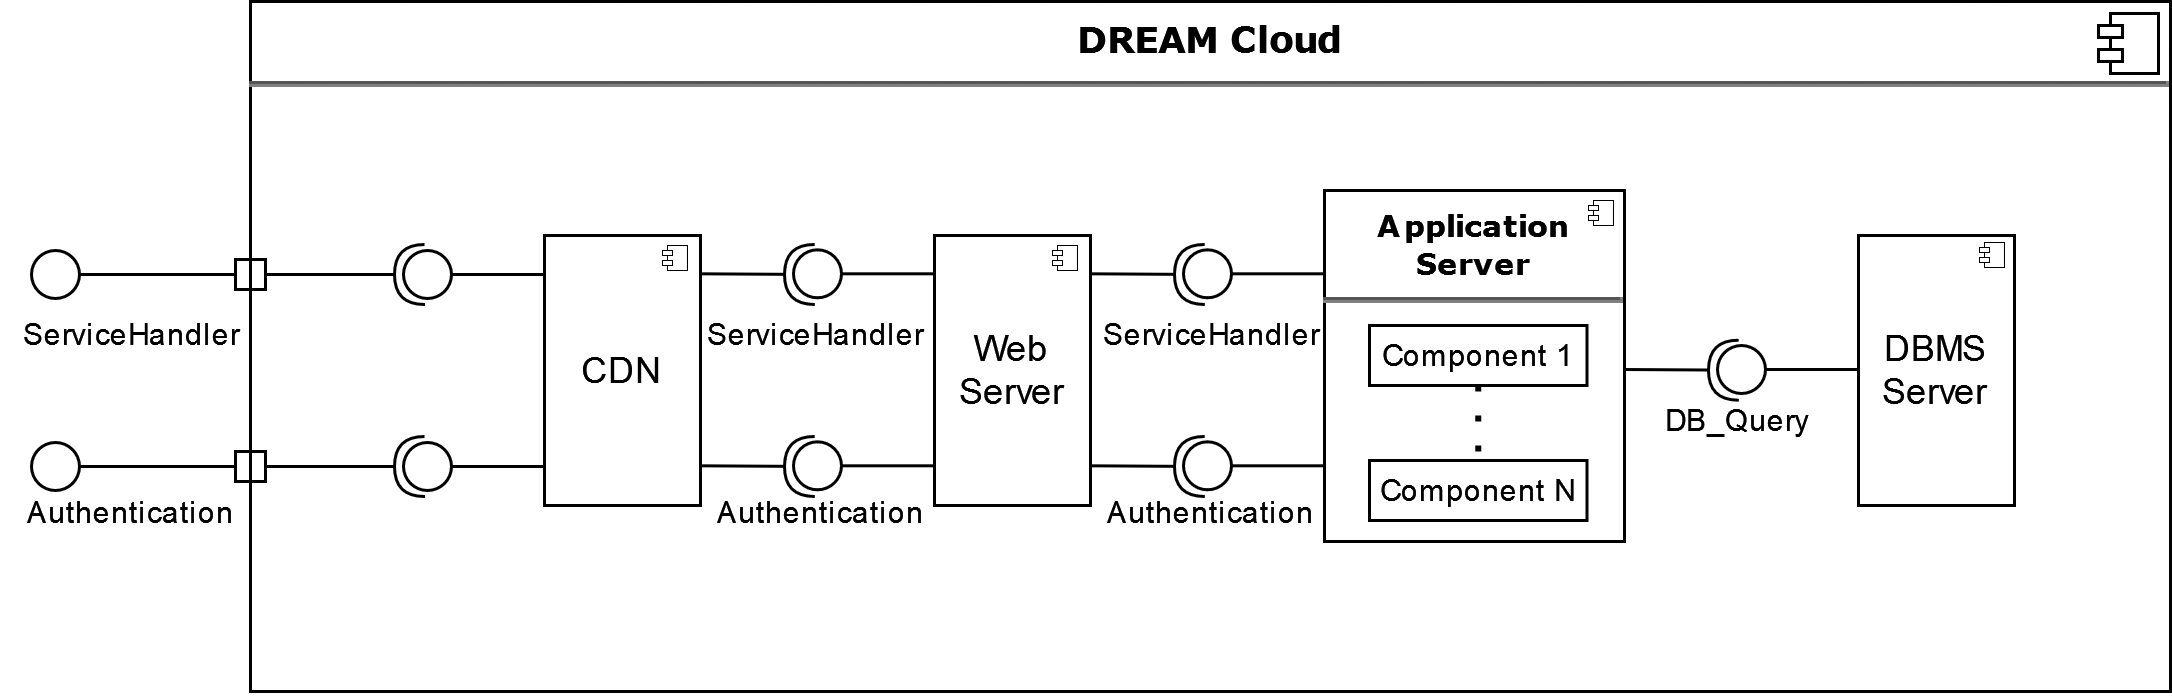
\includegraphics[width=\textwidth]{../images_diagrams/dd/component_only_cloud.png}
\caption{DREAM Cloud Component View.}
\label{fig:CloudOnlyComp}
\end{figure}

The cloud architecture illustrated in Figure \ref{fig:CloudOnlyComp} is based on the following components:
\begin{itemize}
	\item a CDN is implemented as the first component to improve the availability, performance, and redundancy of the entire system
	\item the web server is used to accept the HTTPS requests and send HTTPS responses. It provides static data as well as dynamic data obtained by the application server.
	\item the application server is the main component at this granularity. It contains about 15 smaller components that implement the business logic of the system. The dynamic content of the application is generated here.
	\item the DBMS server is responsible for the storage of data inside a database
\end{itemize}
Aside from the application server, all the others can be implemented using commercial off-the-shelf products (COTS). \\

\subsubsection{Application Server Component}

Figure \ref{fig:ApplicationServerOnlyComp} describes the application server and its components with the highest level of detail, as developers will have to implement the business logic themselves.\\

\begin{figure}[hbt!]
\centering
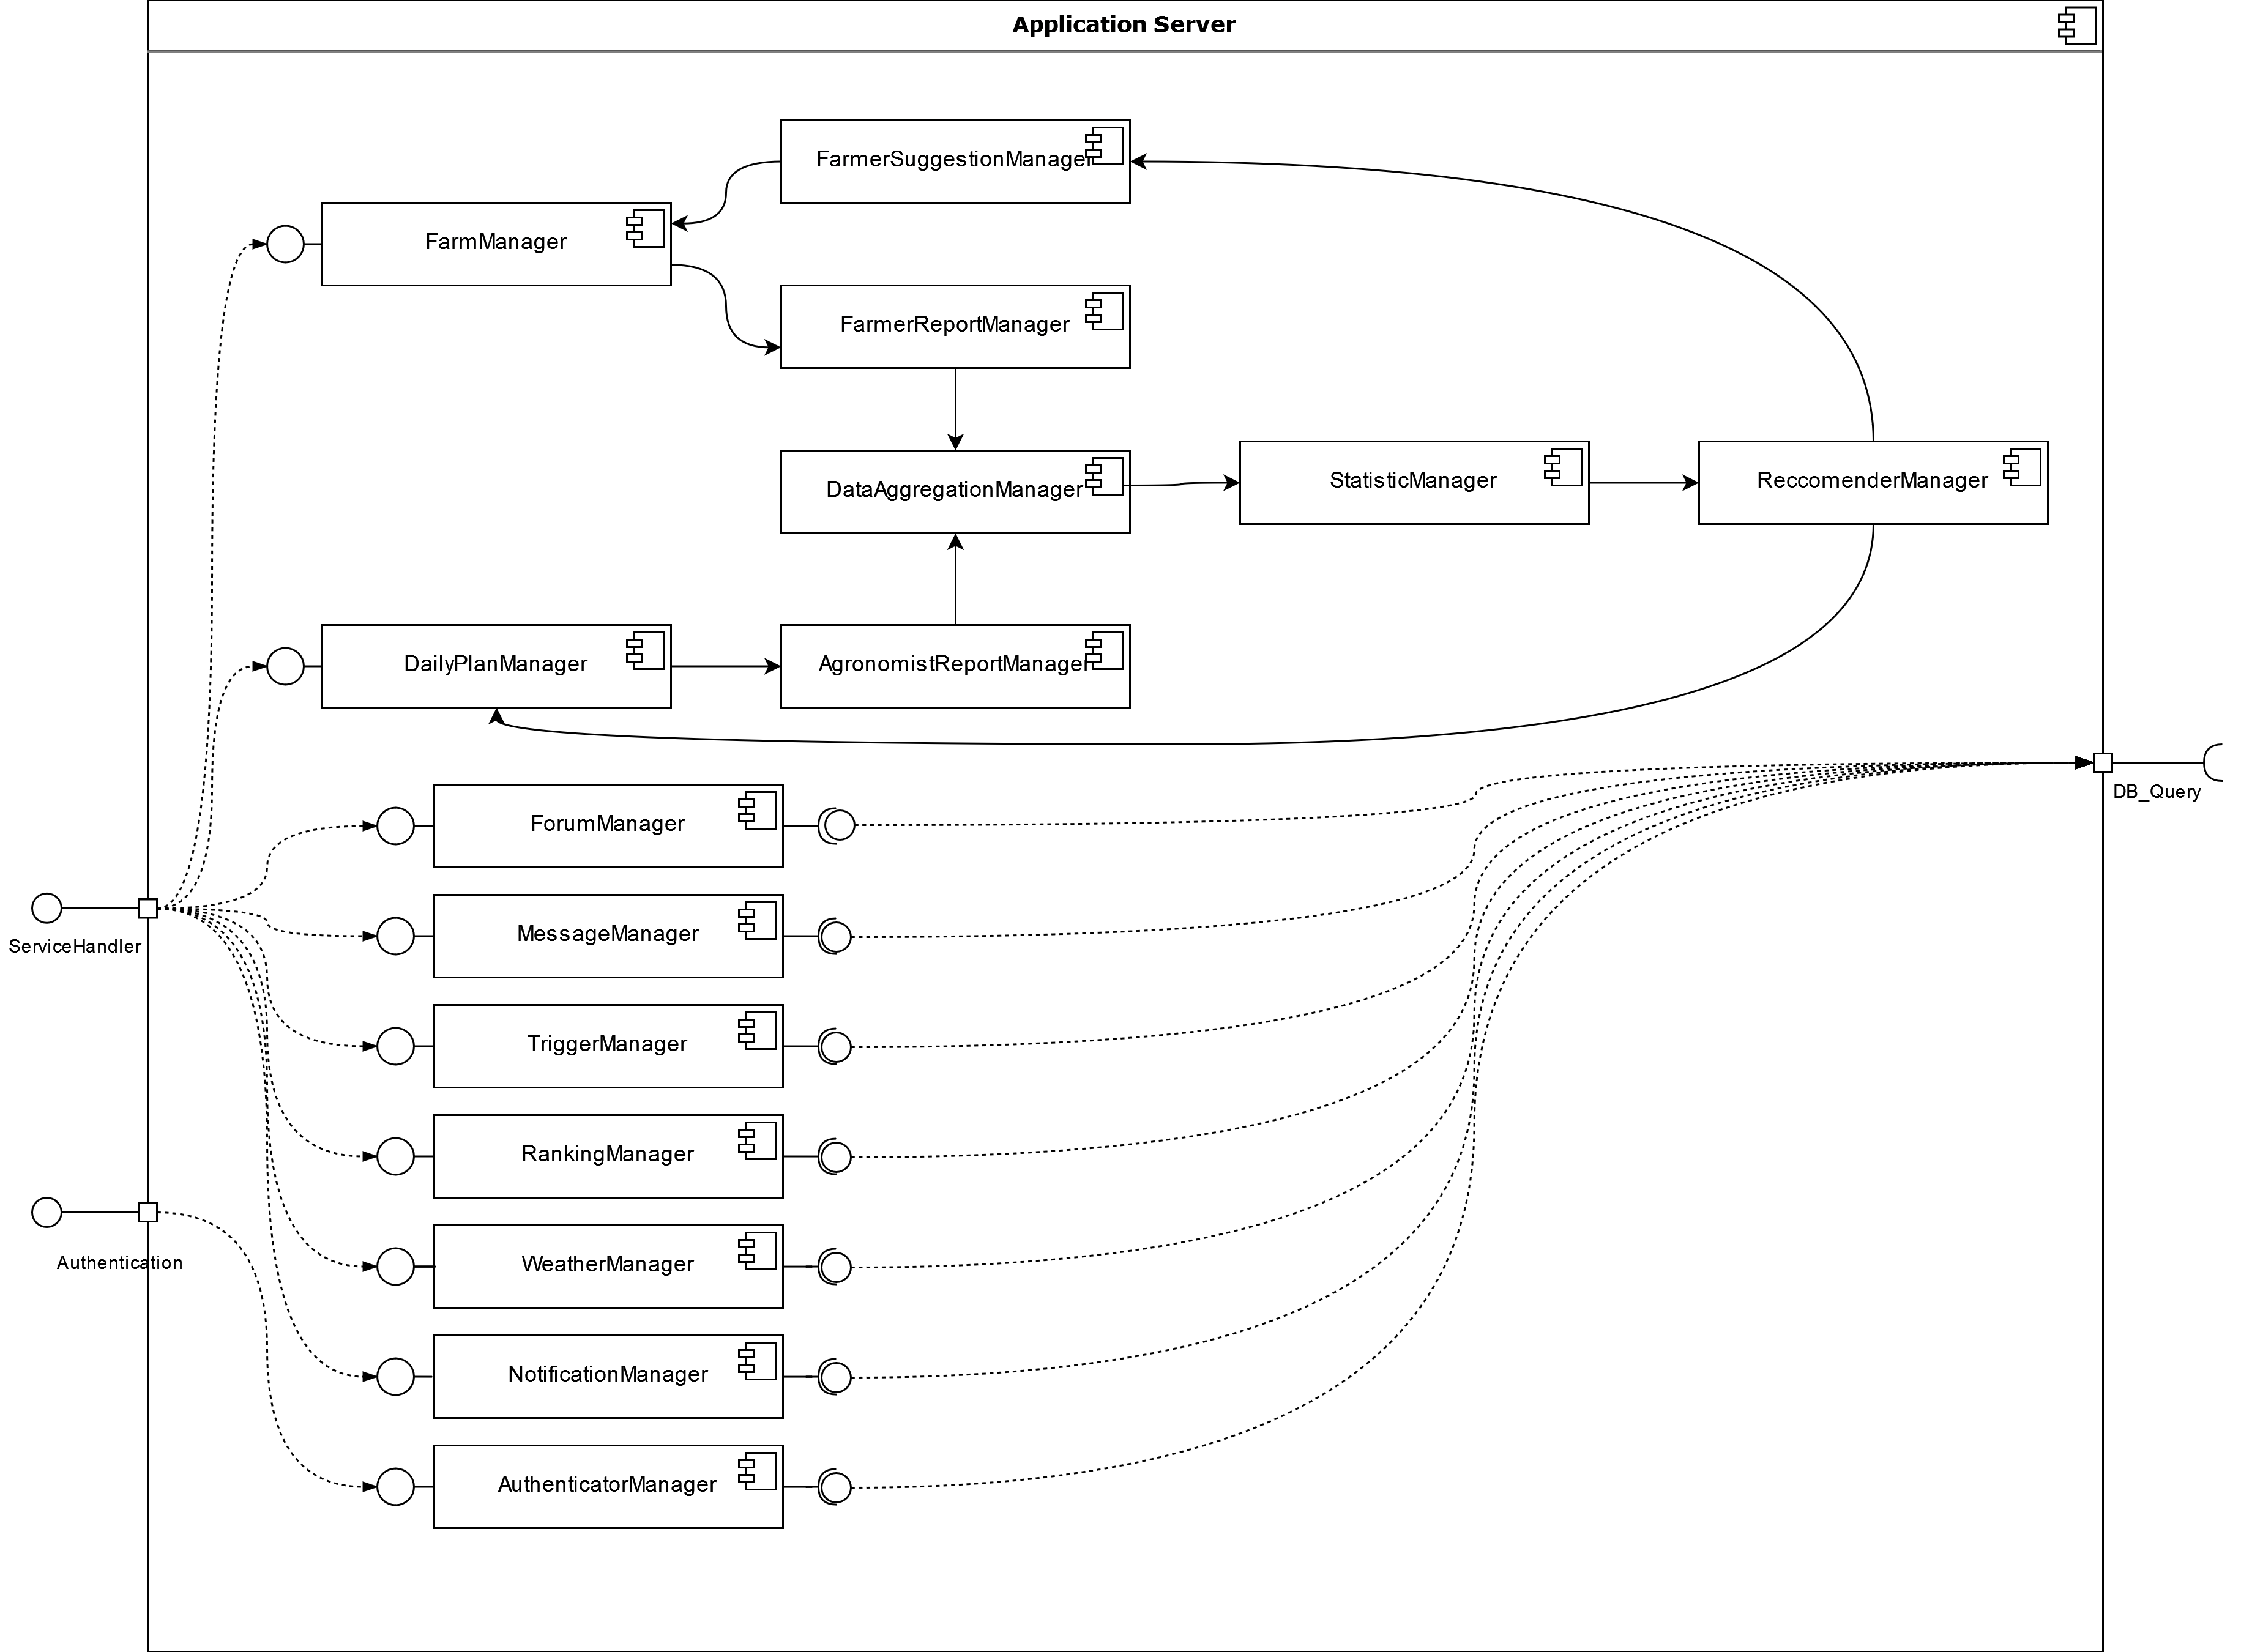
\includegraphics[width=\textwidth]{../images_diagrams/dd/component_only_application.png}
\caption{Application Server Component View.}
\label{fig:ApplicationServerOnlyComp}
\end{figure}

\noindent
The main components in the application server, providing all the business logic in DREAM, are:

\begin{itemize}
	\item The \textbf{AuthenticationManager} is responsible for the login, registration, and logout operations. It allows the users to use their credentials to get access to the application. It is also in charge of the password reset procedure.
	\item The \textbf{ForumManager} manages the Farmer Forum with the creation, deletion, and edits of posts and threads. 
	\item The \textbf{FarmManager} handles the My Farm section in the mobile application, providing the farmer with all the information about their farm and fields.
	\item The \textbf{FarmerReportManager} is in charge of collecting the production data. Other information such as production yields is collected from the farmer and stored inside the database.
	\item The \textbf{AgronomistReportManager} is in charge of collecting data from the agronomist. Data such as production data, a numerical score, and other information about the yields is stored inside the database.
	\item The \textbf{DataAggregationManager} is responsible for aggregating data and information obtained from the reports.
	\item The \textbf{StatisticsManager} manages the calculation of various statistics based on historical data.
	\item The \textbf{RecommenderManager} generates recommendations for farmers and agronomists, based on the previously calculated statistics.
	\item The \textbf{FarmerSuggestionManager} relays suggestions about the production, such as which plant species to plant or the fertilizers to use, to the farmers.
	\item The \textbf{DailyPlanManager} is responsible for the creation, modification, and confirmation of the daily plans.
	\item The \textbf{MessageManager} handles the communication between farmers and agronomists. It collects the message from the sender and forwards it to the recipient.
	\item The \textbf{NotificationManager} module is in charge of sending notifications to users. It is used on different occasions, such as when an agronomist receives a new message from a farmer or when there is a new thread in the Farmer Forum.
	\item The \textbf{TriggerManager} handles the creation, modification, and deletion of triggers by the policy makers. It creates a trigger at the database level, whenever possible, and executes a check for each trigger each time new data is provided through the reports.
	\item The \textbf{RankingManager} is responsible for the creation and update of farmer rankings based on the provided data and calculated statistics.
	\item The \textbf{WeatherManager} collects and provides data about the weather to farmers and agronomists.
\end{itemize}

\subsection{Deployment View}
\begin{figure}[hbt!]
\centering
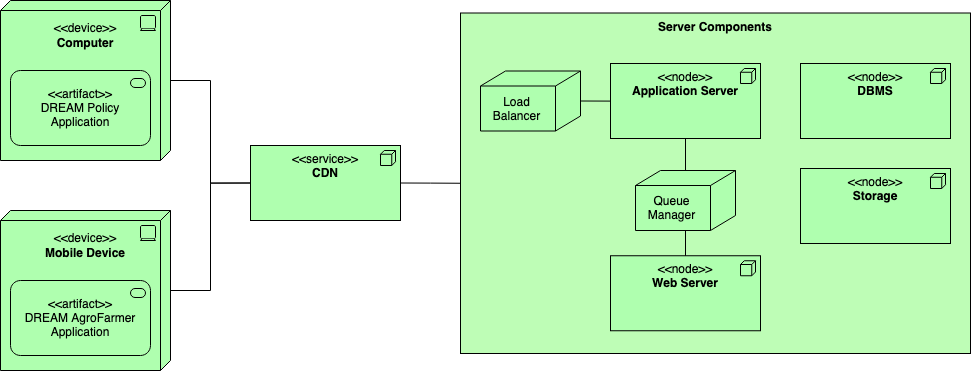
\includegraphics[width=\textwidth]{../images_diagrams/dd/highlevel_deployment.png}
\caption{High-Level Deployment View.}
\label{fig:highLevelDeploy}
\end{figure}

\noindent
The main components in the deployment view in Figure \ref{fig:highLevelDeploy} are the client devices and the cloud platform. Policy makers will access the DREAM Policy Application via a computer device whereas agronomists and farmers will access the DREAM AgroFarmer Application via a mobile device. The CDN is represented as an external service. Then, the server components of the DREAM Cloud include the application server, the web server, the database server, and the load balancer.



\subsection{Runtime View}


\noindent
As shown in the Figure \ref{fig:messagesSequenceDiagram}, when the farmer user accesses the Ask Experts area in the application, the farmer will send a request for help to their assigned agronomist in the form of a message. The agronomist and the farmer can continue to exchange messages until either user chooses to end the conversation. The sequence diagram only represents one message exchanged between them for clarity. The MessageManager has a key role in this interaction; it is the component that communicates with the DBMS for storing data and with the NotificationManager for notifying the other user of the message received.\\


\begin{figure}[hbt!]
\centering
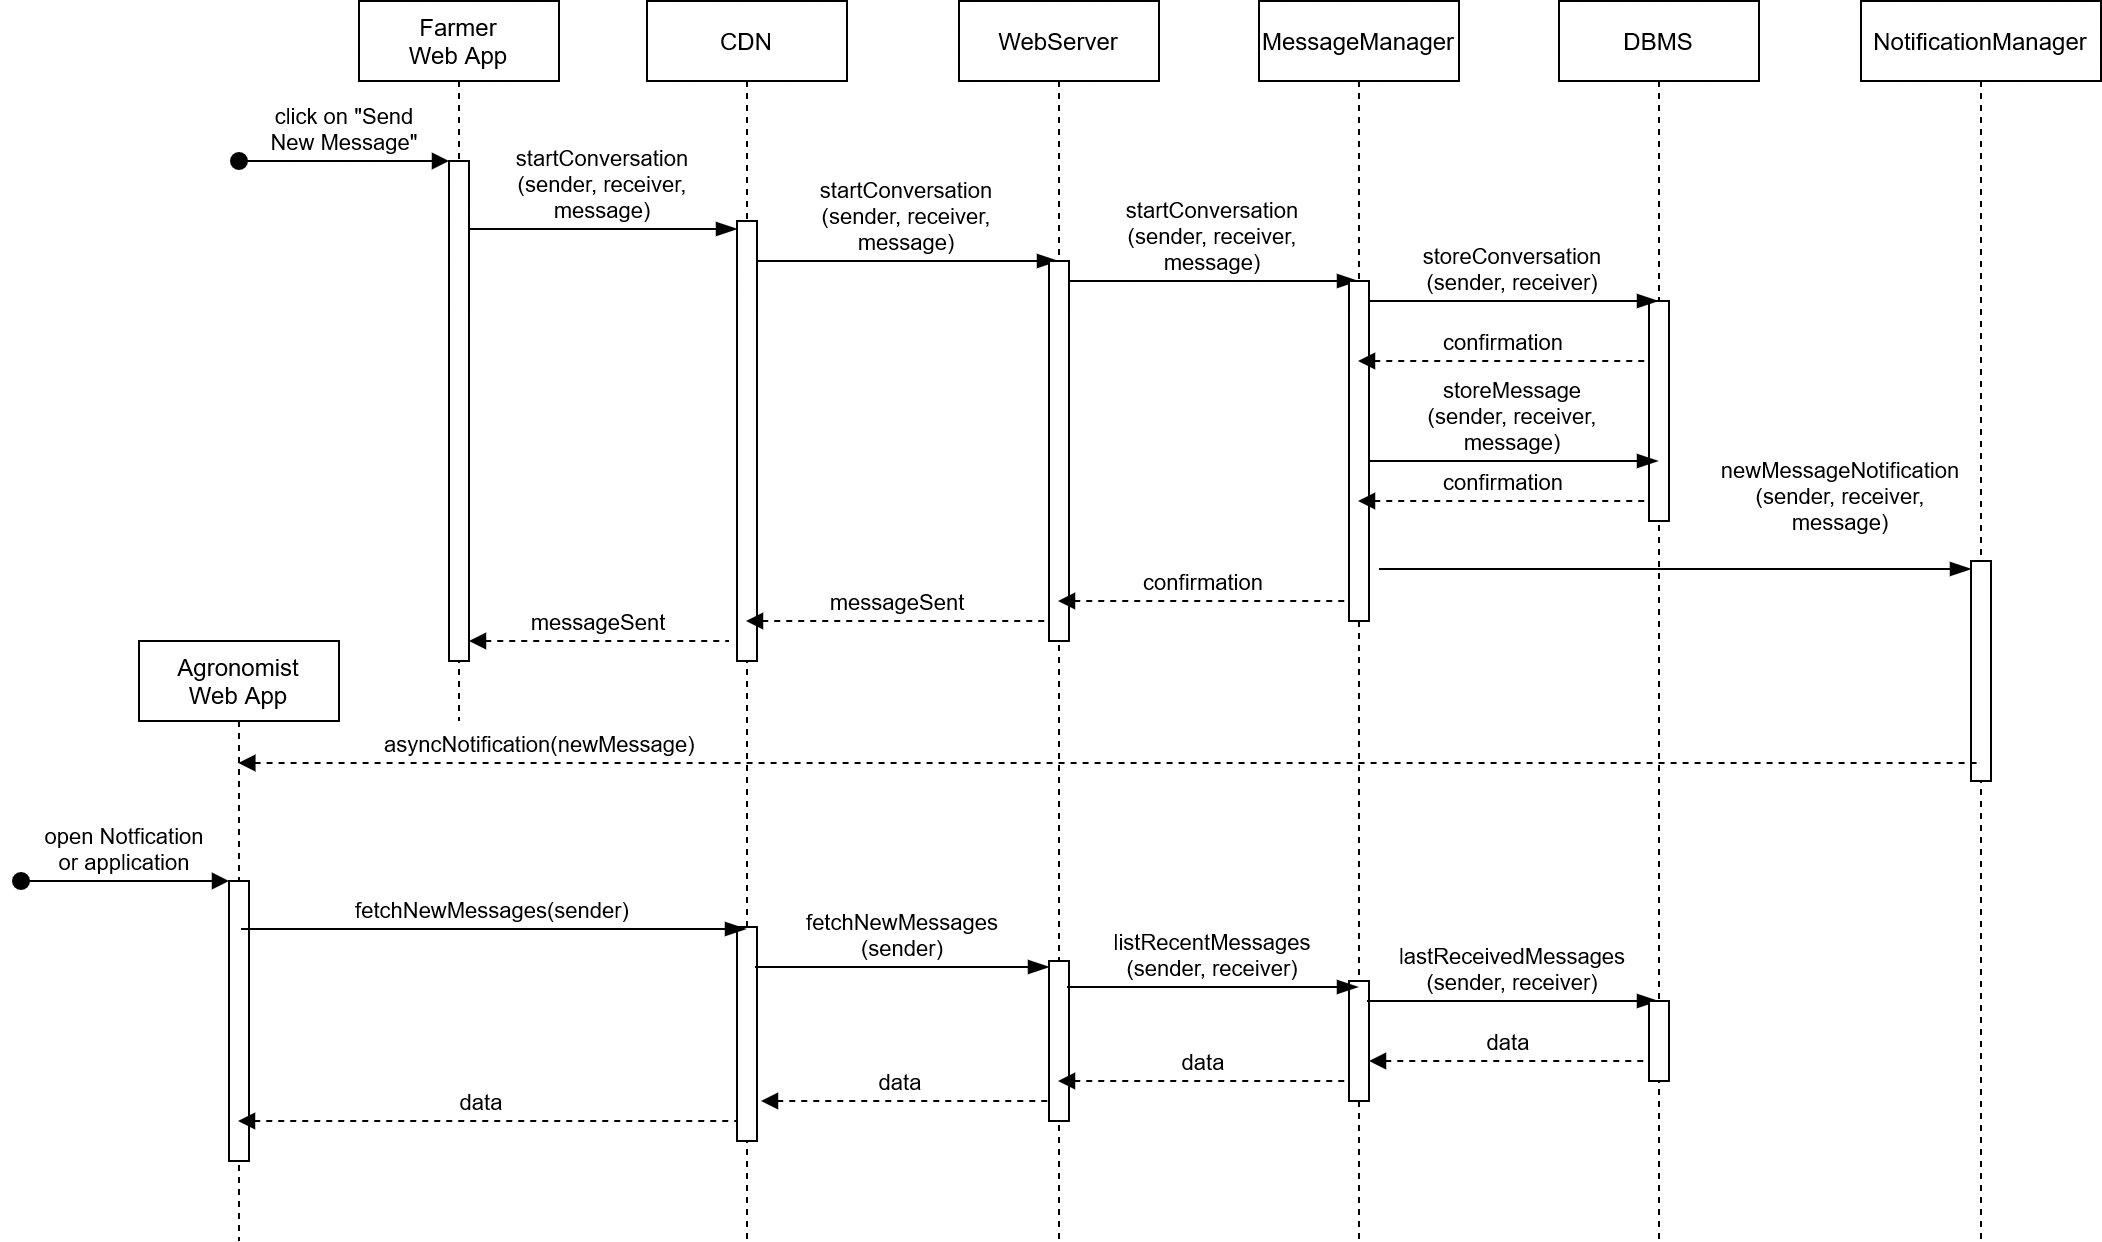
\includegraphics[width=0.9\textwidth]{../images_diagrams/dd/messagesSequenceDiagram.png}
\caption{Messages Sequence Diagram}
\label{fig:messagesSequenceDiagram}
\end{figure}

\noindent
Figure \ref{fig:agronomistDailyPlanSequenceDiagram} represents the daily plan creation performed by an agronomist. The key component this time is the DailyPlanManager. It interfaces with the RecommenderManager that, after retrieving data and statistics by the other components, generates a suggested list of farmers to return to the DailyPlanManager. Then, when it receives the list of suggested farmers, the DailyPlanManager also has to communicate with the Google API to get the path connecting them all. It then stores the daily plan by communicating with the DBMS server.\\

\noindent
Figure \ref{fig:policyMakerRankingSequenceDiagram} represents the actions of viewing the ranking of the farmers and applying a filter to the ranking. The RankingManager is the protagonist of this interaction; it instigates the DataAggregationManager and StatisticManager to retrieve data from all the other components shown in the figure. Then, when it has all the information, it can generate the ranking and returns it to the web application.
Once it has calculated the ranking, it is available for applying filters to it and showing them to the user.\\



\begin{figure}[hbt!]
\centering
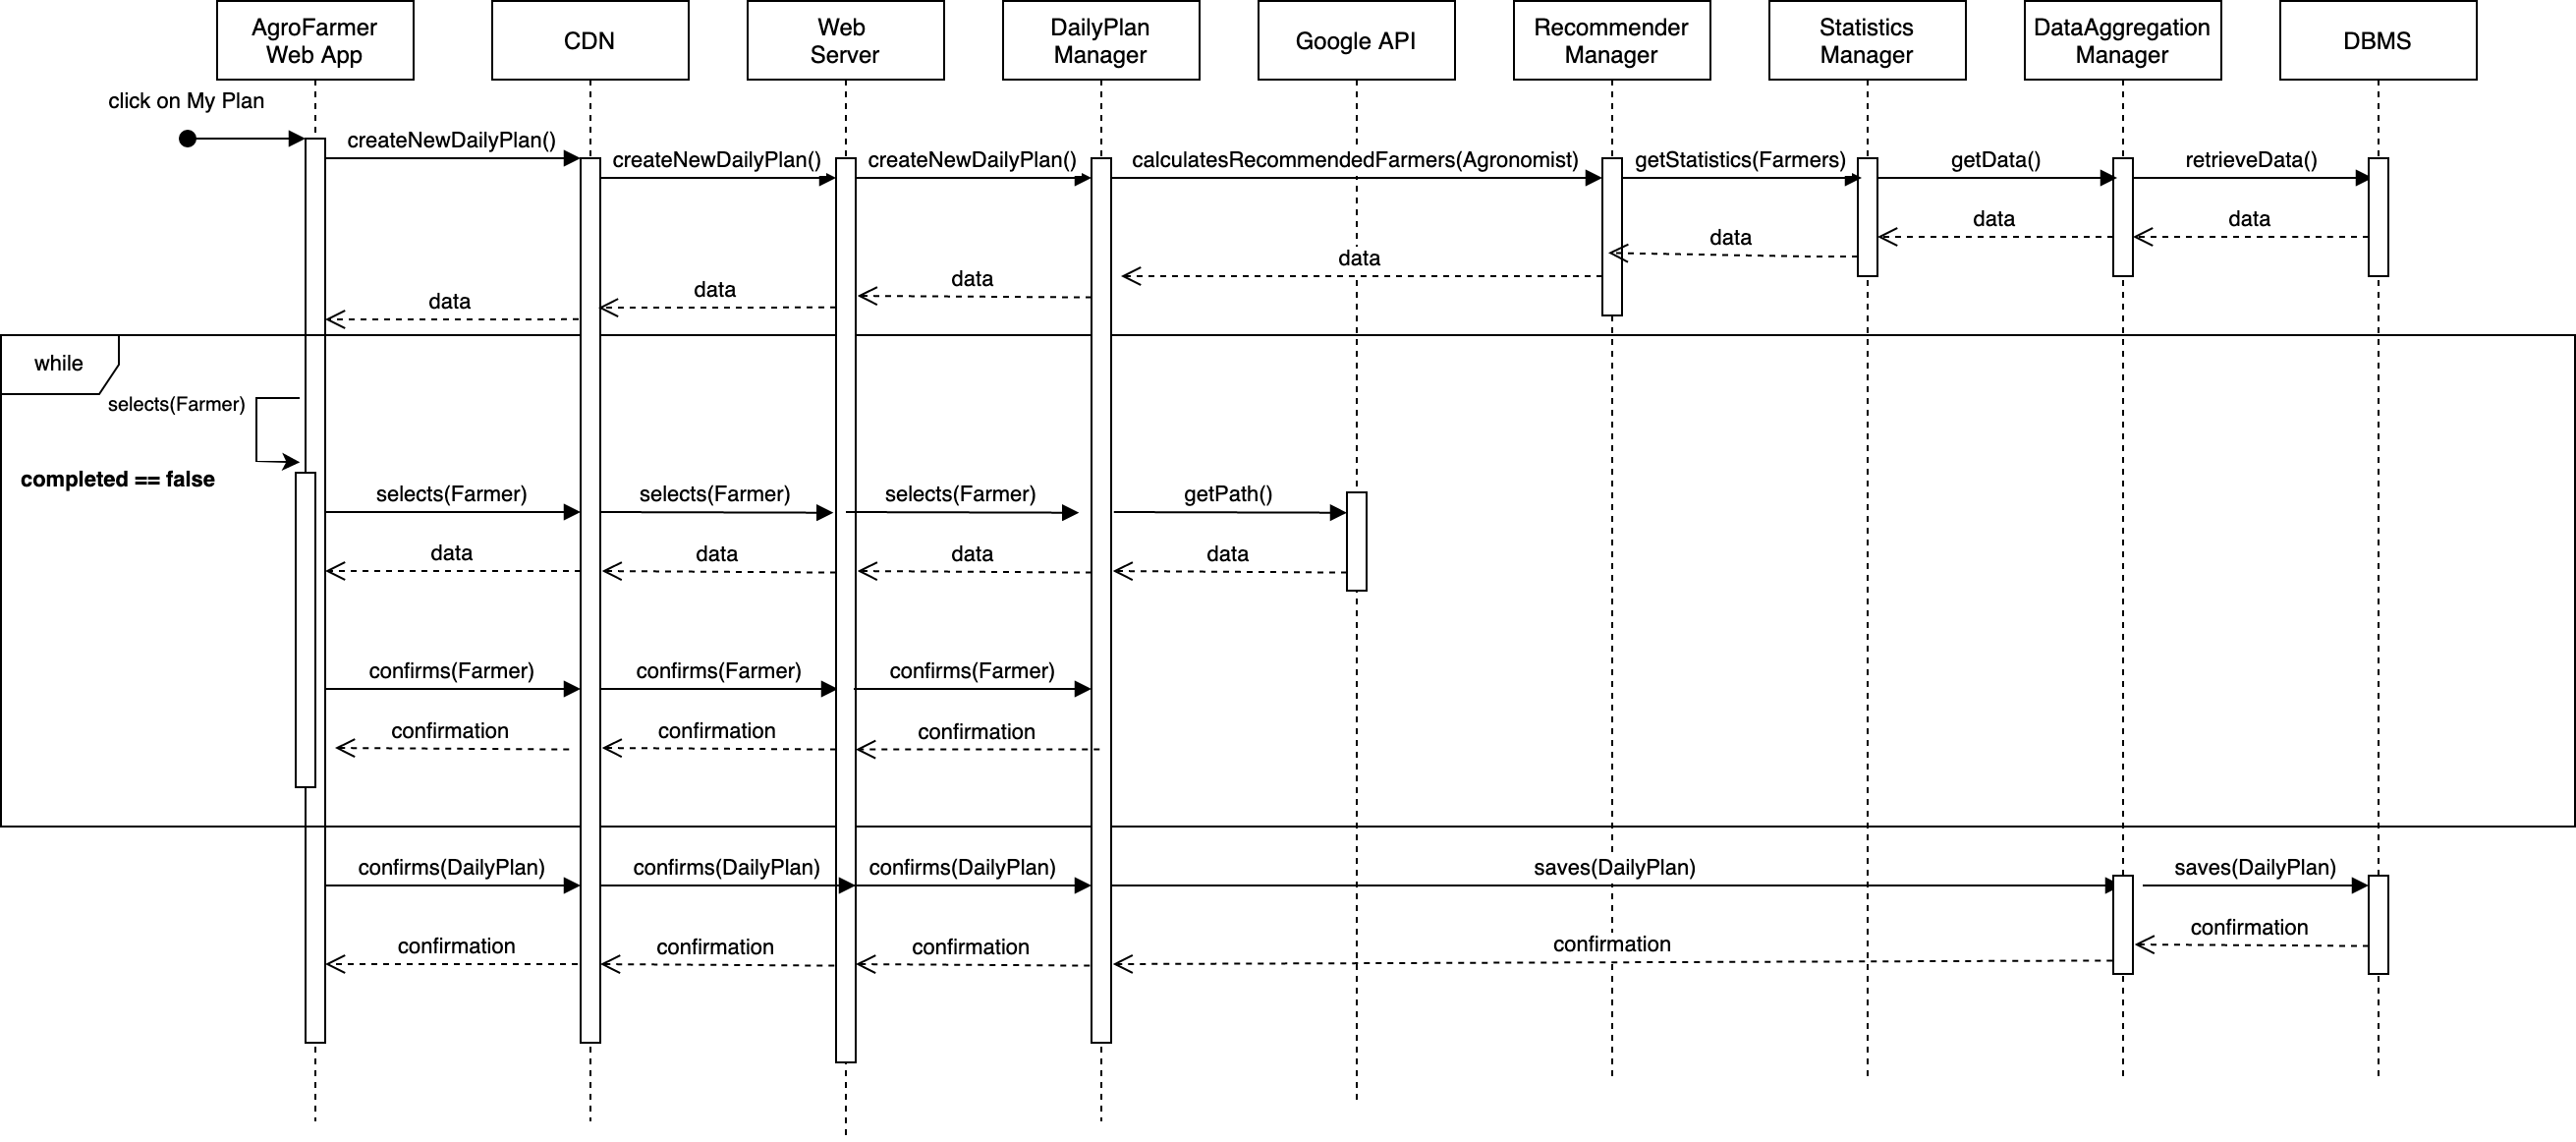
\includegraphics[width=\textwidth]{../images_diagrams/dd/agronomist_sequencediagram.png}
\caption{Agronomist Creating Daily Plan Sequence Diagram}
\label{fig:agronomistDailyPlanSequenceDiagram}
\end{figure}


\begin{figure}[hbt!]
\centering
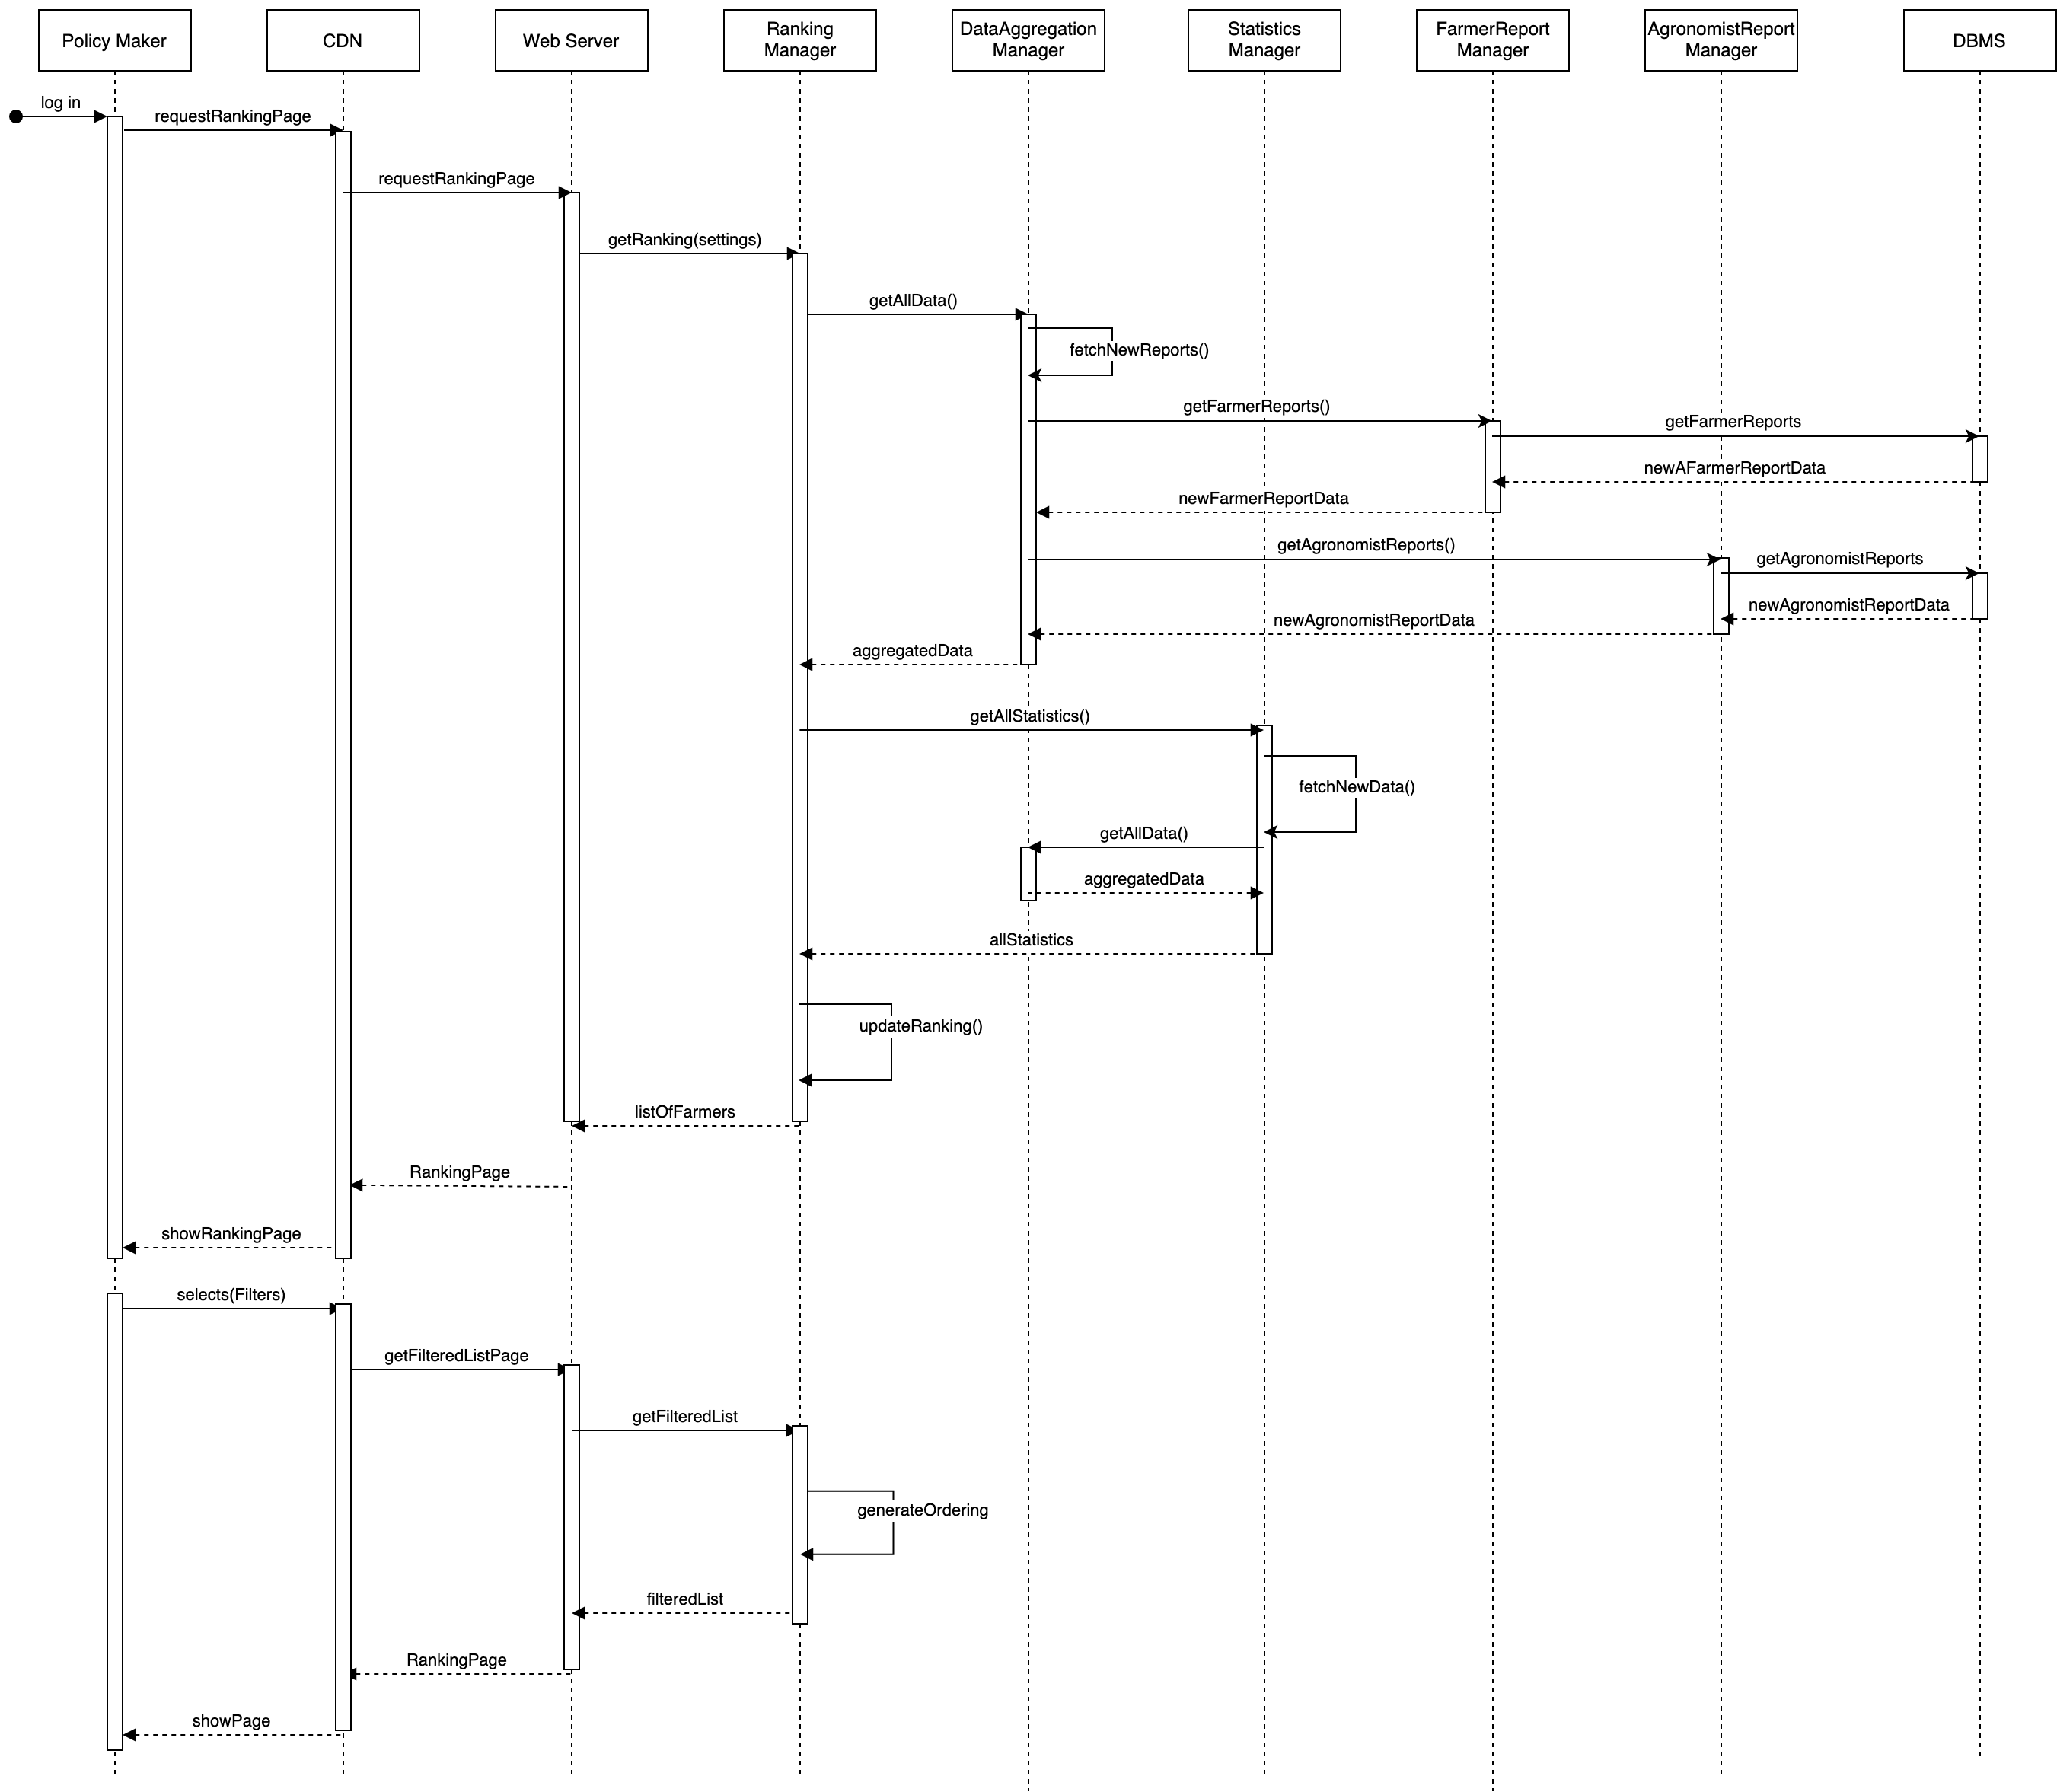
\includegraphics[width=\textwidth]{../images_diagrams/dd/policyMakerSequenceDiaEXT.drawio.png}
\caption{Policy Maker Ranking Sequence Diagram}
\label{fig:policyMakerRankingSequenceDiagram}
\end{figure}

\newpage
\subsection{Component Interfaces}
\noindent
This diagram shows the components of the application server with the main accessible methods.\\

\begin{figure}[H]
\centering
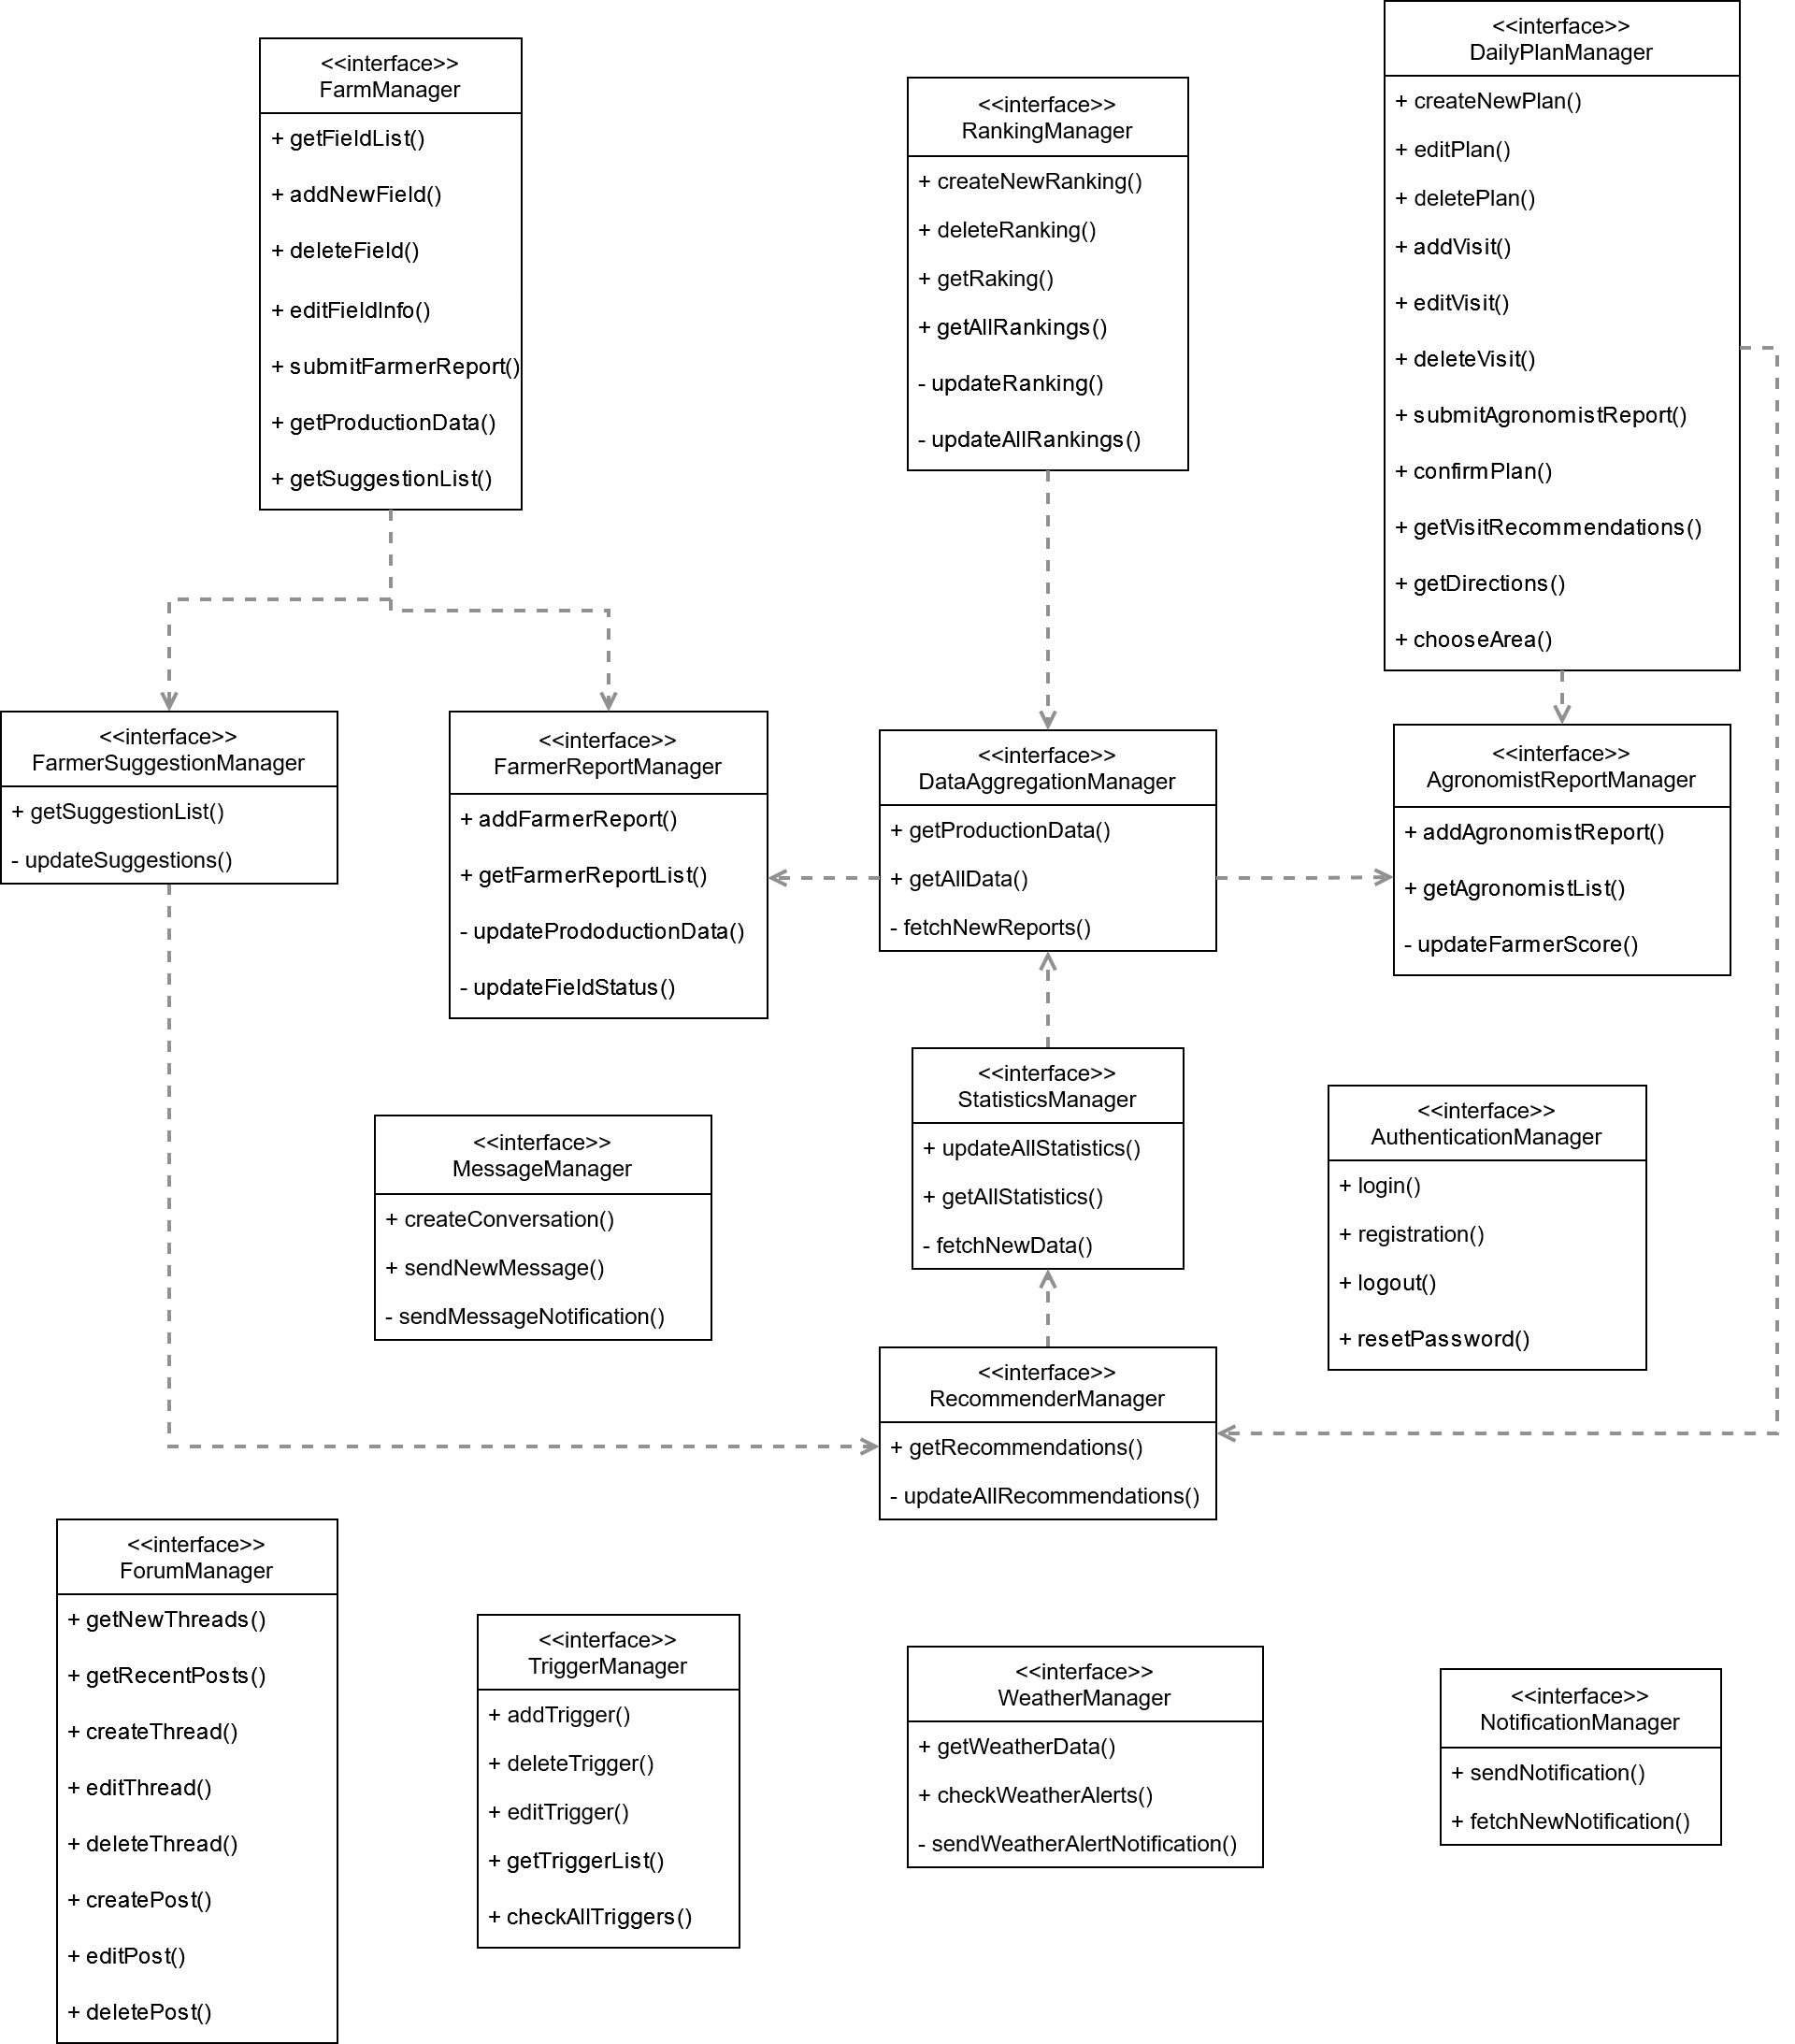
\includegraphics[width=\textwidth]{../images_diagrams/dd/component_interfaces_diagram.png}
\caption{Application Server Component Interfaces Diagram.}
\label{fig:componentInterface}
\end{figure}

\subsection{Selected Architectural Styles and Patterns}
\noindent
As stated in Section \ref{sect:overview}, the system is designed as a \textbf{client-server architecture}, adapted in a \textbf{multi-tiered cloud configuration}. This choice favors, first of all, the decoupling of the system, which maximizes reusability, scalability, and flexibility.\smallskip \\
The presence of only web applications, thus implementing only the presentation layer, is typical of a \textbf{thin client}. The main advantage of such a configuration is the simplified management both for the user, not forced to download any software and for the developers, who can adopt a “write once, run everywhere" approach and push updates to the clients very easily.\smallskip \\
Finally, the architecture uses an \textbf{external CDN} to distribute static content with the highest efficiency and performance. The CDN caches the static contents implemented by the web applications, while it acts as a proxy for the dynamic contents and API requests to the back-end.\\

\subsection{Other Design Decisions}

\subsubsection{Entity–Relationship Model}
\noindent
Figure \ref{fig:ERDiagram} represents an entity-relationship diagram of the database to help the reader identify the key entities and the main relationships and attributes.

\begin{figure}[hbt!]
\centering
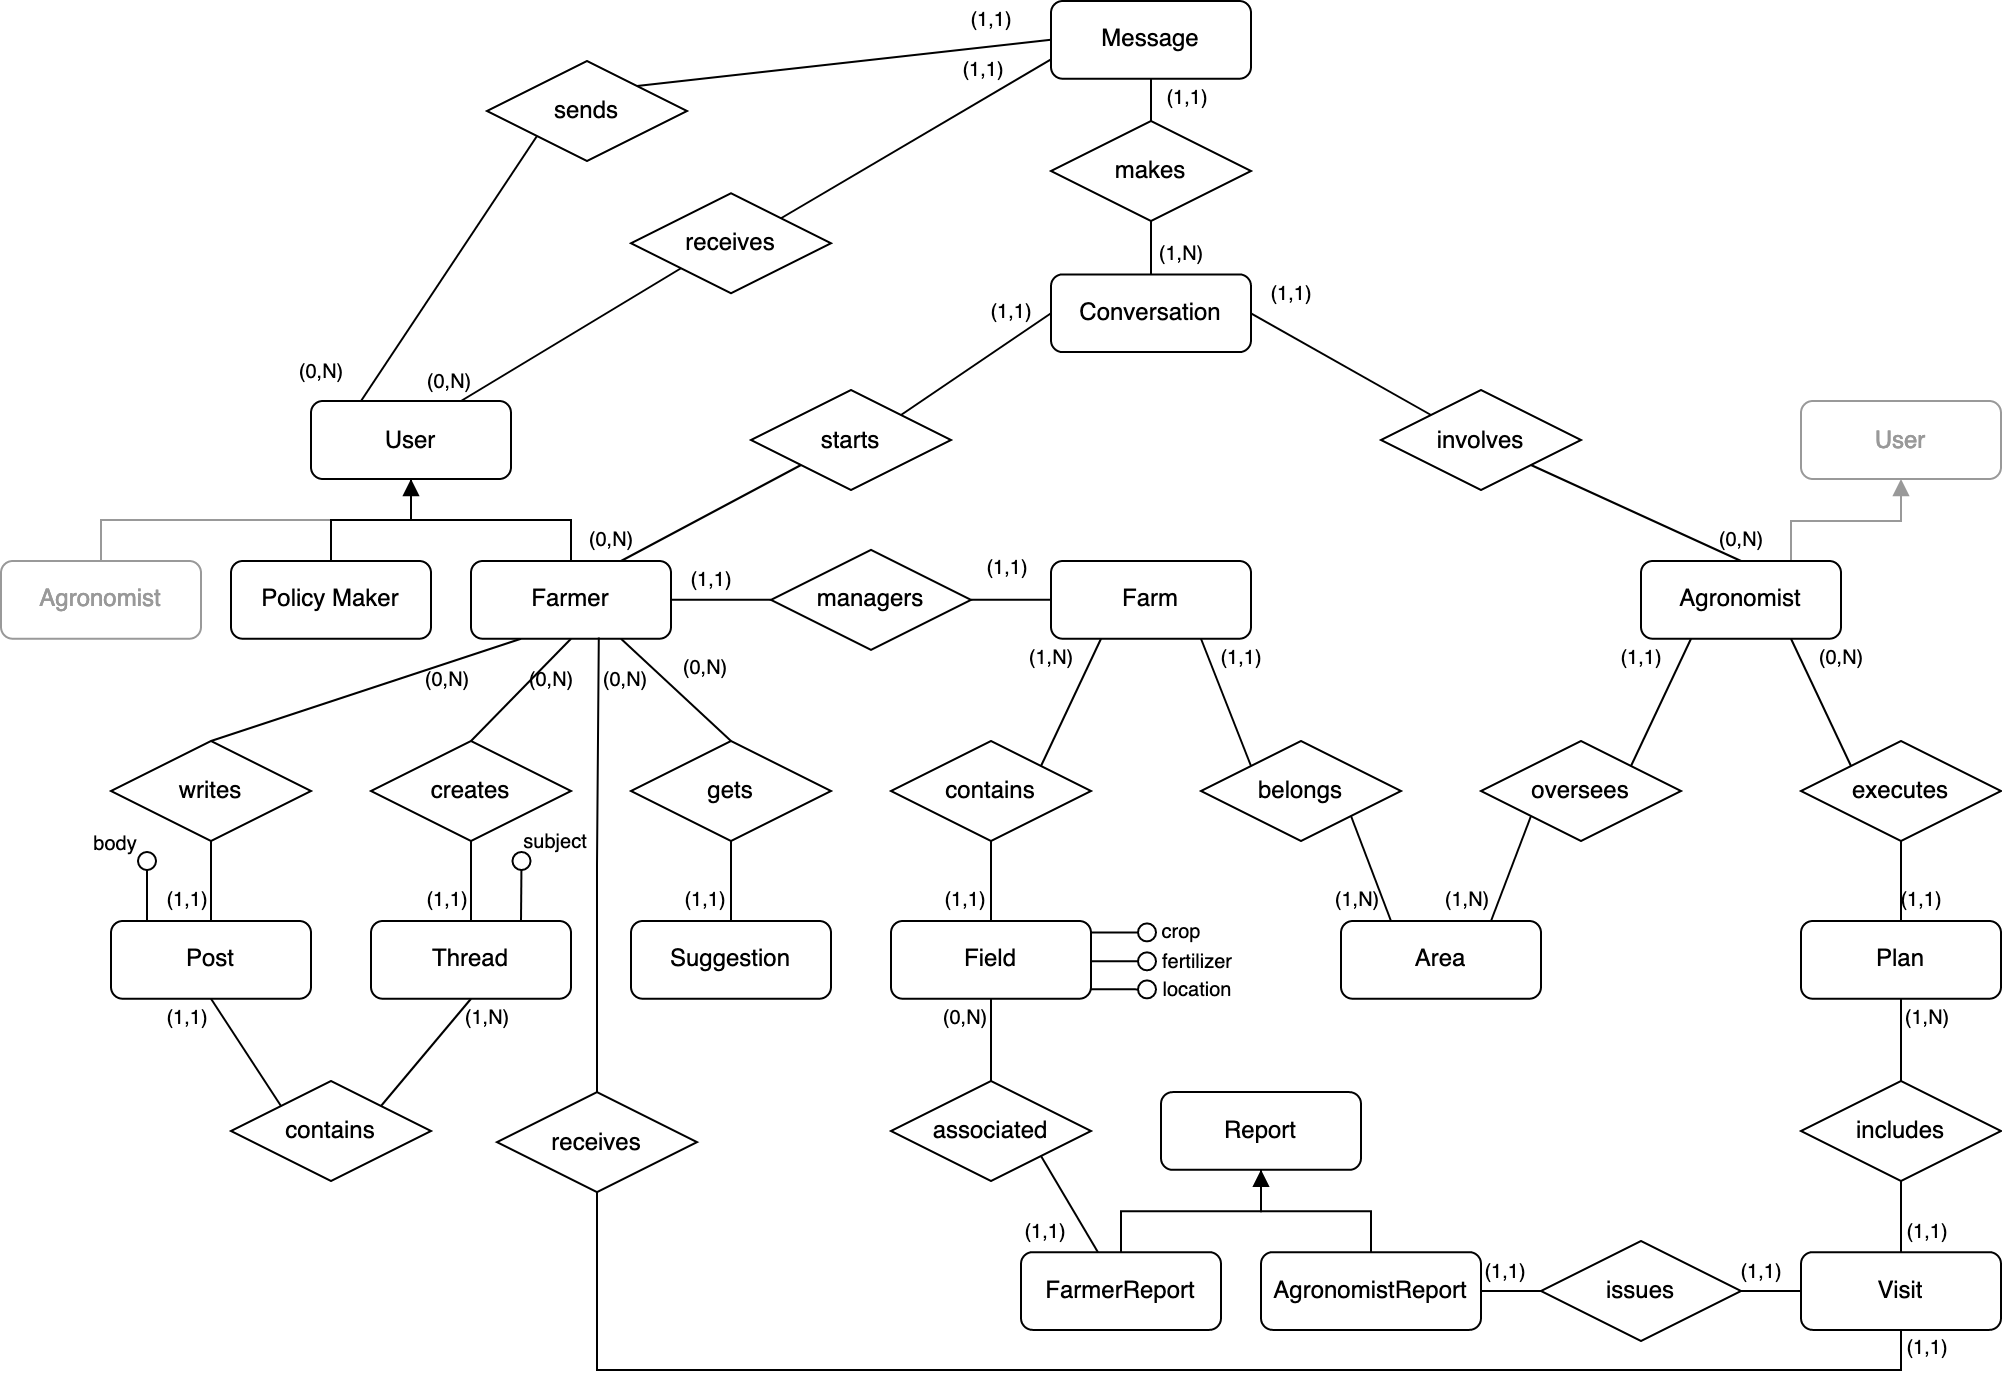
\includegraphics[width=\textwidth]{../images_diagrams/dd/er_diagram.png}
\caption{ER Diagram.}
\label{fig:ERDiagram}
\end{figure}

\noindent
For more graphical clarity, the Agronomist entity is represented twice:
\begin{itemize}
	\item on the left to show the exclusive hierarchy relation between the User, Agronomist, Policy maker, and Farmer entities
	\item on the right with all the other relations. 
\end{itemize}

\noindent
The hierarchy relation between the Report, FarmerReport, and AgronomistReport entities is exclusive. The ER diagram closely follows the relationships as they are described in the Alloy model in the RASD. For graphical clarity, not all the attributes are included in this diagram. Only some interesting attributes, such as crop, fertilizer, and location for the Field entity, are included to specify that such descriptions are attributes instead of entities themselves. Other features of the system such as ranking are not included in this diagram because those are calculated at runtime; only entities related to the database storage are relevant in this diagram.

\subsubsection{HTTPS connection}
\noindent
The communication between the front-end client and the back-end servers is implemented with an encrypted standard such as HTTPS in order to provide a high level of security.
